\documentclass{article}
\usepackage{graphicx} % Required for inserting images
\usepackage[T2A]{fontenc}
\usepackage[english, russian]{babel}

\setlength\parindent{1.5em}


\title{Домашнее задание 4}
\author{Андрей Зотов}
\date{Май 2023}
\begin{document}

\maketitle

\section*{Задача 1}
{\bf Ответ:} 
\begin{itemize}
\item a) Максимальная длина ориентированного простого цикла в графе $G$ равна 3. На графе $G$ всего имеется 6 ориентированных простых циклов длины 3: $A,B,C,A$; $B,C,A,B$; $C,A,B,C$; $A,D,C,A$; $D,C,A,D$; $C,A,D,C$. 
\item б) В графе $G$ всего имеется 3 компоненты сильной связности: $ABCDG$, $E$ и $F$.
\item в) Достаточно добавить одно ориентированное ребро $(F,\ D)$. 
\end{itemize}
{\bf Решение.} в) Как следует из пункта б) чтобы граф $G$ стал сильно связным нужно чтобы существовали ориентированные пути, связывающие (в обе стороны) вершины $E$ и $F$ c компонентой $ABCDG$ (пусть далее это будет компонента $G_1$). При этом вершины $E$ и $F$ тоже будут связаны (в обе стороны). 
\par
Действительно, если добавить ориентированное ребро $(F,\ D)$, то 
\begin{itemize} 
\item Из $E$ в компоненту $G_1$ будет ориентированный путь $E,F,D$. 
\item Из  $G_1$ в $E$ будет ориентированный путь $D,E$.
\item Из $F$ в $G_1$ будет ориентированный путь $F,D$.
\item Из $G_1$ в $F$ будет ориентированный путь $D,E,F$.
\item Из $E$ в $F$ будет ориентированный путь $E,F$.
\item Из $F$ в $E$ будет ориентированный путь $F,D,E$.
\end{itemize}
\par
Таким образом, после добавления ориентированного ребра $(F,\ D)$ существуют ориентированные пути, связывающие любую вершину графа $G$ с любой другой вершиной, т.е. граф $G$ становится сильно связным.
\section*{Задача 2}
{\bf Ответ:} $CABGFDE$ (отсортированная в топологическом порядке последовательность вершин графа $H$).
\section*{Задача 3}
{\bf Ответ:} все собрания получится провести в пятницу. Минимальное количество временных слотов будет 4.
\\
\\
{\bf Решение.} Пусть рабочие группы будут вершинами некоторого графа $G$. При этом вершины графа $G$ связаны ребром, если у соответствующих рабочих групп есть общие участники. Т.е. из условия получаем, что подграфы: $abcd\equiv K_4$, $gfd\equiv K_3$, $bde\equiv K_3$ и $ef\equiv K_2$. Кроме того понятно, что невозможно провести собрание двух рабочих групп в один и тот же слот, если соответствующие вершины графа $G$ связаны ребром. Поэтому первый вопрос задачи равносилен существованию правильной раскраски графа $G$ в 4 цвета. Такая раскраска существует (см. рисунок ниже).
\\
{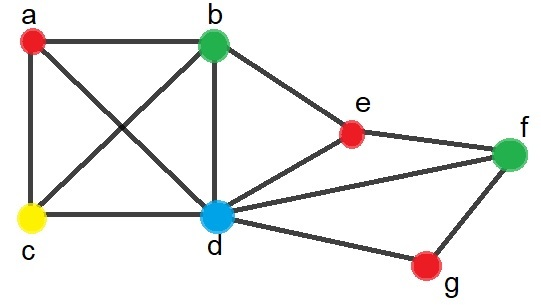
\includegraphics[scale=0.6]{img/img1.jpg}}
\par
Однако меньшим количеством цветов обойтись невозможно, т.к. граф $G$ содержит подграф $abcd$, который эквивалентен $K_4$, а для $K_4$ необходимо для правильной раскраски ровно 4 цвета. Т.е. 4 временных слота - это минимальное количество необходимое для планирования собраний.
\section*{Задача 4}
{\bf Ответ:}  а) $mk$; б) $n^2$.
\\
\\
{\bf Решение.} a) В простом двудольном графе любую белую вершину можно соединить со всеми черными, тогда из каждой белой вершины будет выходить максимально возможное число ребер - по $m$ штук  (кратные ребра не рассматриваем). Т.к. всего белых вершин $k$ штук, то всего ребер будет $mk$ штук. (Cимметрично можно было бы рассматривать $m$ черных вершин, где из каждой выходит максимальное число ребер - по $k$ штук и получается тоже самое максимальное число ребер $mk$).
\par б) Т.к. рассматривается двудольный граф, то все его вершины можно разбить на два класса - черные и белые, при этом каждое ребро графа соединяет вершины из разных классов. Пусть белых вершин будет $k$ штук, тогда черных будет $2n-k$ штук. Согласно пункту а) максимально возможное число ребер при заданном $k$ будет $M_k=k(2n-k)$ штук.
\par
Найдем $k$, при котором $M_k$ достигает максимума. Заметим, что $$M_k=n^2 - (n-k)^2$$
Как видно $M_k$ достигает максимума $n^2$, когда второе отрицательное слагаемое обращается в ноль, т.е. при $k=n$. 
\par
Таким образом, максимальное число ребер двудольного графа достигается, когда черных и белых вершин по $n$ штук, а максимальное число ребер будет $n^2$.
\section*{Задача 5}
{\bf Ответ:}  a) слово $aaabbbabaa$; б) не существует.
\\
\\
{\bf Доказательство.} a) Рассмотрим ориентированный граф $G$, в качестве вершин которого будут выступать трехбуквенные комбинации (всего 8 штук), а ориентированные ребра будут связывать начальную комбинацию $\alpha_1\alpha_2\alpha_3$ с конечной комбинацией $\beta_1\beta_2\beta_3$, если комбинацию $\alpha_1\alpha_2\alpha_3$ можно продолжить буквой $\alpha_4$, так что $\alpha_2\alpha_3\alpha_4\equiv \beta_1\beta_2\beta_3$. Тогда существование слова по условию п. a) будет равносильно существованию $\textit{простого}$ ориентированного пути в графе $G$, который содержит все вершины графа $G$. Рассмотрим этот граф (рисунок ниже).
\\
{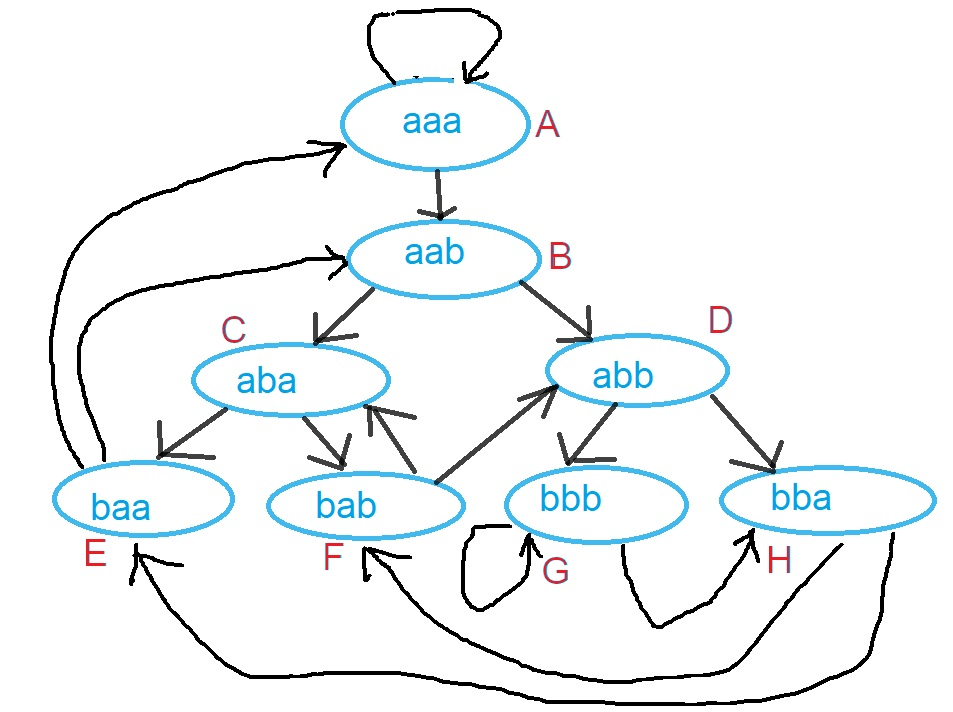
\includegraphics[scale=0.3]{img/img2.jpg}}
\\
На рисунке вершины графа $G$ обозначены большими латинскими буквами. И как видно существует простой ориентированный путь $A,B,D,G,H,F,C,E$, который содержит все вершины графа. Слово, которое соответствует этому пути будет $aaabbbabaa$.
\par
{\bf Решение.} б) Слово, которое начиналось бы на $abba$ и удовлетворяло бы условию п. а) не существует. Потому что иначе существовал бы простой ориентированный путь в графе $G$, содержащий все вершины графа, где первая вершина была бы $D$ (комбинация $abb$), а вторая $H$ (комбинация $bba$). Но это невозможно, т.к. этот путь обязан содержать кроме прочих вершину $G$ (комбинация $bbb$), а в эту вершину можно попасть либо из нее самой, либо из вершины $D$. Т.е. искомый путь должен содержать 2 вершины $D$, а значит он не является простым.
\end{document}